%% This is an example first chapter.  You should put chapter/appendix that you
%% write into a separate file, and add a line \include{yourfilename} to
%% main.tex, where `yourfilename.tex' is the name of the chapter/appendix file.
%% You can process specific files by typing their names in at the 
%% \files=
%% prompt when you run the file main.tex through LaTeX.
\chapter{Introduction}\label{intro-ch}

\section{Distributed Systems}


With the rise of big data, new data processing systems have been designed to help process it. 
Instead of relying on using just onemore powerful computers, these systems use many computers and are thus distributed in nature due to economic costs,scalability, and fault tolerance. Because programming in these  distributed environments is challenging, data processing systems
try to abstract this from the user and provide a simple interface for them. One of the most popular systems is Map Reduce,
invented by Google, which provides a simple map and reduce operation to the user. Another of these systems is Spark, which provides
a slightly more expressive api then map reduce and also has different modes of fault tolerance than spark along with caching. 
One key and slow stage that both of these systems have, is that because they are distributed in nature, they have a stage
where data must be transferred between machines, called the shuffle stage. This shuffle stage can be the bottleneck and be the reason for low performance of jobs.
\section{Shuffle} 

In map reduce, data is loaded onto different computers and an computation is performed on it (the map phase) that results 
in a group of key value pairs. The final phase of map reduce,the reduce phase assumes that all key-value pairs with the same
key are grouped onto the same machine. Thus, an intermediate phase that these systems handle themselves is the shuffle phase where
data is transferred so that all key value pairs with the same keys result to be on the same machine. 
\\

The following example in Figure~\ref{fig:shuffle_basic} details the inner workings 
of what happens in a shuffle for map reducer. Suppose we want to count the 
number of letters in a distributed file. The mappers will count the number of
letters in their individual file. However, we need to aggregate this and 
thus all the counts for letter a will be sent to worker1, letter b will be sent to worker 2,
letter c will be sent to worker c. These reducers will then promptly aggregate the counts that they receive from the 
mappers.

\begin{figure}[h]
\begin{center}
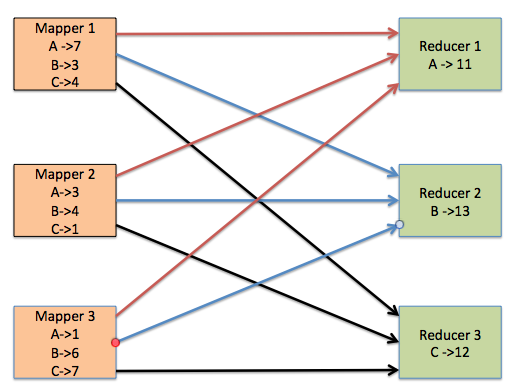
\includegraphics[scale=1.0]{./img/shuffle_basic.png}
\caption{Shuffle for Letter Count in Map Reduce. The red arrows represent the transfer of the A key,
the blue arrow represents the transfer of the B key, and the black arrows represents the transfer of the C key}
\label{fig:shuffle_basic}
\end{center}
\end{figure}

Because of the huge amounts of keys, these systems do not deal with on the granurality of keys.
nstead, they deal with the concepts of partitions. These systems have different partitioning functions
that map key-value pairs to different partitions. Some popular partition schemes include range and hash partitioning.
As long as all the mappers agree to partition their data in the same way and send each partition that is the same to the same reducer, we are ensured that any two keys that are the same will be in the same partition. 

\section{Overview of EEG Analysis}\label{intro-ch:eeg-overview}

A seizure is a transient aberration in the brain's electrical activity. People
with the central nervous system disorder epilepsy suffer from recurrent
seizures, often happening suddenly and at unpredictable times. A seizure can
vary from a lapse of attention to a whole-body convulsion. Frequent seizures
are dangerous, as they can increase risk of sustaining physical injuries and
can even result in death \cite{eeg-ml}. \\

One method for detecting the onset of epileptic seizures is the analysis of
scalp EEG data, a non-invasive measure of the brain's electrical activity.
Continuous EEG (cEEG) data is typically recorded using 19 silver/silver
chloride electrodes, affixed to the scalp \cite{ceeg-1}.
Figure~\ref{fig:electrodes} shows a drawing of the placement of sensors on a
patient's scalp. \\

\begin{figure}[h]
\begin{center}
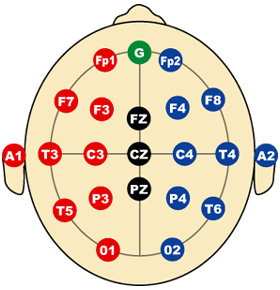
\includegraphics[scale=0.5]{./img/electrodes.png}
\caption{EEG electrode placement on a patient's scalp.}
\label{fig:electrodes}
\end{center}
\end{figure}

Trained individuals, such as attending physicians, epilepsy/neurophysiology
fellows, or registered EEG technicians (encephalographers), review and screen
EEG recordings, which typically take place over a continuous 24-hour period
\cite{ceeg-3}. Unlike traditional epilepsy monitoring units which focus on
provoking and capturing seizures, the goal of cEEG studies is to efficiently
identify future seizures and prevent them. This leads to an increase in the
number of cEEG recordings for preventative measures. Intensive care unit
centers are subsequently overwhelmed with the analysis of the growing dataset
due to the small number of available trained individuals. Methods to screen
long EEG recordings without sacrificing accuracy are necessary to be able to
efficiently process this data. \\

Typically, EEGs displays show no more than 10 to 15 seconds of data per screen
of raw voltage readings and requires an analyst to simultaneously inspect
multiple channels. In contrast, a compressed spectral array \cite{csa} or
spectrogram display may show 2 to 8 hours of data on a single color map
\cite{ceeg-3}. This allows analysts to quickly screen long periods of EEG data,
determining which segments, if any, require direct review of the raw data.
Spectrogram review reduces cEEG review time by $78\%$ \cite{ceeg-2}, with
minimal loss of sensitivity compared with conventional review. For these
reasons, we focus on building a tool to rapidly analyze spectrogram data. \\

\begin{figure}[h]
\begin{center}
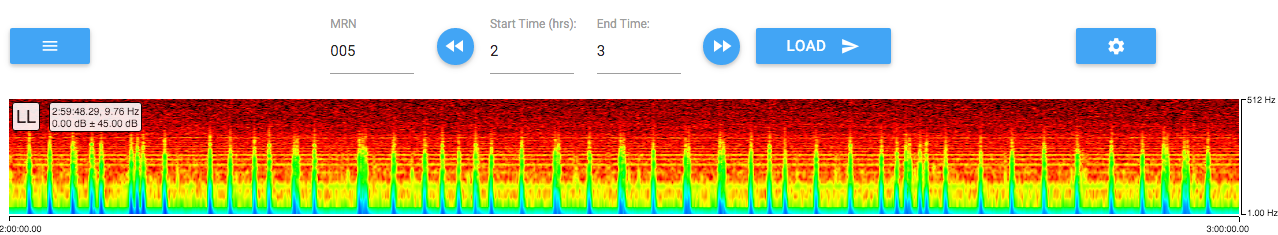
\includegraphics[scale=0.35]{./img/eeg-view.png}
\caption{Spectrogram for one hour window of EEG data of the \c{LL} region of
  the brain.}
\label{fig:eeg-view}
\end{center}
\end{figure}

Spectrograms are the most widely used compressed data format for EEG data
\cite{ceeg-1}. A spectrogram consists of three-dimensional plots with time on
the x-axis, frequency on the y-axis, and EEG power on the z-axis.
Figure~\ref{fig:eeg-view} shows an example of rendered spectrogram data. An
analyst typically views four spectrograms concurrently, mapped to different
regions of the brain. Each region is formed by using multiple EEG channels
where an EEG channel is the difference between voltages measured at two
electrodes. This captures the summed potential of millions of neurons
\cite{eeg-ml}.  Figure~\ref{fig:electrodes} shows the electrode placement on
the patient's scalp, yielding four regions for analysis: left lateral power,
\c{LL}, (Fp1-F7, F7-T3, T3-T5, T5-O1), left parasagittal power, \c{LP},
(Fp1-F3, F3-C3, C3-P3, P3-O1), right lateral power, \c{RL}, (Fp2-F8, F8-T4,
T4-T6, T6-O2), right parasagittal power, \c{RP}, (Fp1-F4, F3-C4, C4-P4, P4-O2).
\\

Data from a single patient can vary in size from tens to hundreds of gigabytes
and the number of EEG tests performed each year is estimated to be between 10
and 25 million \cite{eeg-scale}. As this corpus of data collected at the ICU
continues to grow, efficient mechanisms to store and visualize this data at
scale are key for analysts to quickly view patient screenings. Pinky aims to
provide this for analysts by giving them a simple yet powerful interface to
view spectrogram data.

\section{System Architecture}

Pinky is comprised of three coupled layers which handle storage, computation
and visualization. Figure~\ref{fig:system-architecture} shows the overall
architecture of the system.

\begin{figure}[h]
\begin{center}
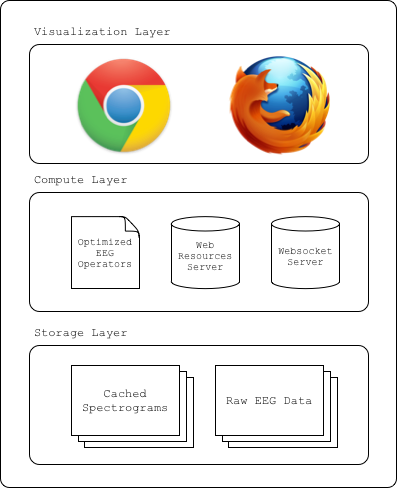
\includegraphics[scale=0.75]{./img/system-architecture.png}
\caption{Pinky system architecture.}
\label{fig:system-architecture}
\end{center}
\end{figure}

\subsection{Storage Layer}

The storage layer, discussed in detail in Chapter~\ref{storage-ch}, is
responsible for storing raw EEG patient data and the calculated spectrogram.
This datastore must optimize both reads and writes of array based data for
multidimensional arrays on the order of tens to hundreds of gigabytes.

\subsection{Compute Layer}

The compute layer, discussed in detail in Chapter~\ref{compute-ch}, is an
extensible module which handles the algorithms to calculate the spectrogram and
other EEG related calculations. As we discuss in
Section~\ref{discuss-ch:future-work}, there are a number of extensions the
project can take, thus it is important that an interested developer can easily
add functionality to this layer. In addition, the compute layer contains two
servers. One server interfaces with the optimized EEG algorithms and the
storage layer to serve array based data. The second server is a lightweight
server for the web resources of the visualization layer.

\subsection{Visualization Layer}

The visualization layer, discussed in detail in Chapter~\ref{viz-ch}, is a browser
based module that renders the data to the client. The interface allows users to
query based on a patient's id (medical record number, \c{mrn}) and view a spectrogram
for a given time interval. An analyst may smoothly pan and zoom throughout the dataset.

\subsection{Visgoth System}

Since enabling interactivity is an important design criteria, we have designed
and built an optimization module for browser based visualizations named
Visgoth. The system uses profiling information from the client and server to
suggest an adaptive scaling of the visualizations served in order to keep
latency consistent, regardless of a client's hardware or network bandwidth. We
discuss Visgoth in detail in Chapter~\ref{visgoth-ch}.

\section{Usage}

The project code base is available publicly on Github \cite{github} at
\url{https://github.com/joshblum/eeg-toolkit}, with documentation for
installing the project for development. In addition, we have created Docker
\cite{docker} images that can easily be installed for production use. Armed
with a dataset, any curious doctor is able to install the images and load the
data for analysis. The docker images are available for public use on DockerHub:
\url{https://hub.docker.com/r/joshblum/eeg-toolkit-webapp} and
\url{https://hub.docker.com/r/joshblum/eeg-toolkit-toolkit}. The Github project
contains specific installation instructions.

\section{Contributions}

Pinky makes the following contributions:

\begin{itemize}

  \item Implements an abstraction for array based storage systems.

  \item Implements three different backends which adhere to the abstraction.

  \item Evaluates the different backends for varying input ranges and
    workloads.

  \item Implements optimized algorithms for analyzing EEG data.

  \item Provides an extensible framework for accessing array based data and
    visualizing it in the browser.

  \item Implements scalable in-browser visualizations using the client's GPU.

  \item Implements a new system, Visgoth, for reducing latency for browser
    based visualizations.

\end{itemize}

These contributions enable doctors and medical expert analysts to interactively
analyze EEG data at scale.

